\documentclass[a4paper,10pt,twocolumn]{ltjarticle}
\usepackage{kaitoushu}

% グラフ用の共通スタイル定義
\pgfplotsset{
  myaxis/.style={
    axis lines=middle,
    xlabel={$x$}, ylabel={$y$},
    every axis x label/.style={at={(ticklabel* cs:1)},anchor=west},
    every axis y label/.style={at={(ticklabel* cs:1)},anchor=south},
    tick label style={font=\scriptsize},
    label style={font=\small},
    width=5.5cm, height=5cm,
    grid=none,
    samples=100,
  }
}

\begin{document}

\problemrange{3章：関数とグラフ — Basic (p.37)（問171--179）}



\mondai{171}{次の関数について，偶関数か奇関数かを調べよ．}
\kotae{
$f(-x)=f(x)$ → 偶（$y$軸対称），$f(-x)=-f(x)$ → 奇（原点対称）．

(1) $3x^{2}$ → 偶\quad
(2) $x-1$ → どちらでもない\quad
(3) $-2x$ → 奇

(4) $x^{2}+x$ → どちらでもない\quad
(5) $x^{4}+5x^{2}-3$ → 偶

(6) $(x-1)^{5}$ → どちらでもない\quad
(7) $\dfrac{1}{4}x^{3}$ → 奇

(8) $\dfrac{1}{x^{2}}$ → 偶\quad
(9) $\dfrac{(x^{2}+3)^{2}}{x}$ → 奇
}

\mondai{172}{次の関数のグラフをかけ．}
\kotae{
基本関数 $y=x^{n}$ の平行移動・反転で描く．

(1) $y=(x-1)^{3}+2$：変曲点$(1,2)$

\begin{tikzpicture}
\begin{axis}[myaxis, xmin=-1.5,xmax=3.5,ymin=-3,ymax=7]
\addplot[thick,blue,domain=-1:3]{(x-1)^3+2};
\addplot[only marks,mark=*,mark size=1.5pt] coordinates {(1,2)};
\node[font=\scriptsize,right] at (axis cs:1,2.5) {$(1,2)$};
\end{axis}
\end{tikzpicture}

(2) $y=-(x+1)^{3}+2$：変曲点$(-1,2)$

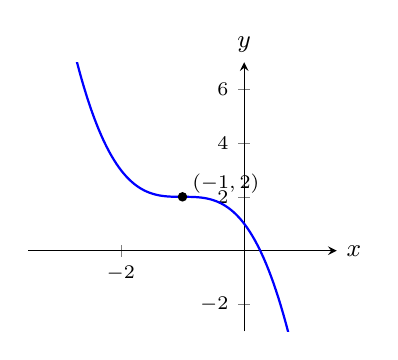
\begin{tikzpicture}
\begin{axis}[myaxis, xmin=-3.5,xmax=1.5,ymin=-3,ymax=7]
\addplot[thick,blue,domain=-3:1]{-(x+1)^3+2};
\addplot[only marks,mark=*,mark size=1.5pt] coordinates {(-1,2)};
\node[font=\scriptsize,right] at (axis cs:-1,2.5) {$(-1,2)$};
\end{axis}
\end{tikzpicture}

(3) $y=(x+1)^{4}-2$：最小点$(-1,-2)$

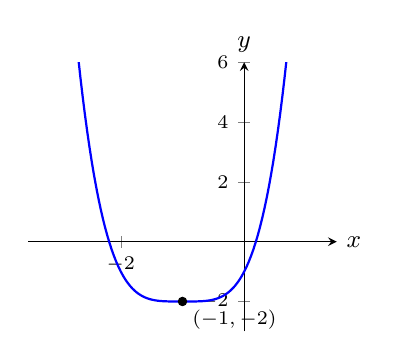
\begin{tikzpicture}
\begin{axis}[myaxis, xmin=-3.5,xmax=1.5,ymin=-3,ymax=6]
\addplot[thick,blue,domain=-2.8:0.8]{(x+1)^4-2};
\addplot[only marks,mark=*,mark size=1.5pt] coordinates {(-1,-2)};
\node[font=\scriptsize,right] at (axis cs:-1,-2.6) {$(-1,-2)$};
\end{axis}
\end{tikzpicture}

(4) $y=-(x-2)^{4}+1$：最大点$(2,1)$

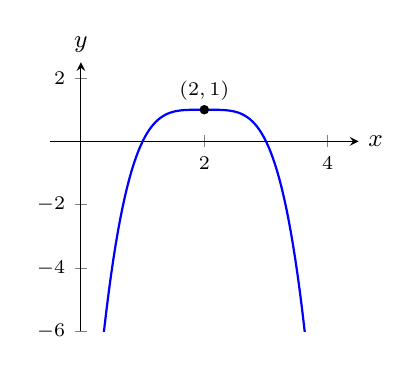
\begin{tikzpicture}
\begin{axis}[myaxis, xmin=-0.5,xmax=4.5,ymin=-6,ymax=2.5]
\addplot[thick,blue,domain=0.2:3.8]{-(x-2)^4+1};
\addplot[only marks,mark=*,mark size=1.5pt] coordinates {(2,1)};
\node[font=\scriptsize,above] at (axis cs:2,1) {$(2,1)$};
\end{axis}
\end{tikzpicture}
}

\mondai{173}{次の関数の定義域と値域を求め，グラフをかけ．また，漸近線を求めよ．}
\kotae{
$y=\dfrac{k}{x-p}+q$ → 漸近線 $x=p$，$y=q$．

(1) $y=\dfrac{1}{x-2}+1$\quad 漸近線：$x=2$，$y=1$

\begin{tikzpicture}
\begin{axis}[myaxis, xmin=-2,xmax=6,ymin=-4,ymax=6,
  restrict y to domain=-10:10]
\addplot[thick,blue,domain=-1.5:1.7,samples=60]{1/(x-2)+1};
\addplot[thick,blue,domain=2.3:5.5,samples=60]{1/(x-2)+1};
\addplot[dashed,red] coordinates {(2,-4)(2,6)};
\addplot[dashed,red] coordinates {(-2,1)(6,1)};
\end{axis}
\end{tikzpicture}

(2) $y=\dfrac{2}{x+1}-2$\quad 漸近線：$x=-1$，$y=-2$

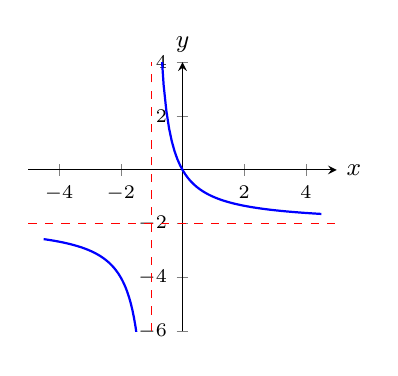
\begin{tikzpicture}
\begin{axis}[myaxis, xmin=-5,xmax=5,ymin=-6,ymax=4,
  restrict y to domain=-10:10]
\addplot[thick,blue,domain=-4.5:-1.3,samples=60]{2/(x+1)-2};
\addplot[thick,blue,domain=-0.7:4.5,samples=60]{2/(x+1)-2};
\addplot[dashed,red] coordinates {(-1,-6)(-1,4)};
\addplot[dashed,red] coordinates {(-5,-2)(5,-2)};
\end{axis}
\end{tikzpicture}

(3) $y=-\dfrac{1}{x-3}+1$\quad 漸近線：$x=3$，$y=1$

\begin{tikzpicture}
\begin{axis}[myaxis, xmin=-1,xmax=7,ymin=-4,ymax=6,
  restrict y to domain=-10:10]
\addplot[thick,blue,domain=-0.5:2.7,samples=60]{-1/(x-3)+1};
\addplot[thick,blue,domain=3.3:6.5,samples=60]{-1/(x-3)+1};
\addplot[dashed,red] coordinates {(3,-4)(3,6)};
\addplot[dashed,red] coordinates {(-1,1)(7,1)};
\end{axis}
\end{tikzpicture}
}

\mondai{174}{次の関数のグラフをかけ．また，定義域と値域および漸近線を求めよ．}
\kotae{
分子÷分母で帯分数に変形する．

(1) $y=\dfrac{x+3}{x+1}=1+\dfrac{2}{x+1}$\quad 漸近線：$x=-1$，$y=1$

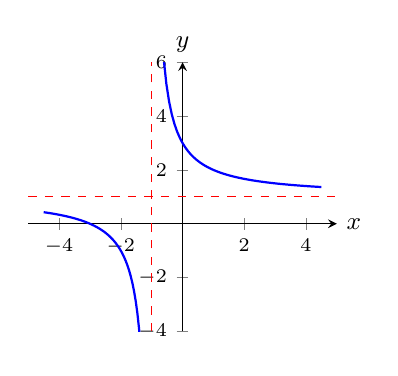
\begin{tikzpicture}
\begin{axis}[myaxis, xmin=-5,xmax=5,ymin=-4,ymax=6,
  restrict y to domain=-10:10]
\addplot[thick,blue,domain=-4.5:-1.3,samples=60]{(x+3)/(x+1)};
\addplot[thick,blue,domain=-0.7:4.5,samples=60]{(x+3)/(x+1)};
\addplot[dashed,red] coordinates {(-1,-4)(-1,6)};
\addplot[dashed,red] coordinates {(-5,1)(5,1)};
\end{axis}
\end{tikzpicture}

(2) $y=\dfrac{2x-5}{x-2}=2-\dfrac{1}{x-2}$\quad 漸近線：$x=2$，$y=2$

\begin{tikzpicture}
\begin{axis}[myaxis, xmin=-2,xmax=6,ymin=-4,ymax=8,
  restrict y to domain=-10:10]
\addplot[thick,blue,domain=-1.5:1.7,samples=60]{(2*x-5)/(x-2)};
\addplot[thick,blue,domain=2.3:5.5,samples=60]{(2*x-5)/(x-2)};
\addplot[dashed,red] coordinates {(2,-4)(2,8)};
\addplot[dashed,red] coordinates {(-2,2)(6,2)};
\end{axis}
\end{tikzpicture}
}

\mondai{175}{次の関数の定義域を求めよ．}
\kotae{
(1) $\sqrt{x-2}$：$x\geqq2$\quad
(2) $\dfrac{-3}{\sqrt{x+1}}$：$x>-1$\quad
(3) $\sqrt{-x^{2}+x+6}$：$-2\leqq x\leqq 3$
}

\mondai{176}{次の関数の定義域と値域を求め，グラフをかけ．}
\kotae{
$y=\sqrt{x}$ の平行移動で考える．

(1) $y=\sqrt{x-2}$：始点$(2,0)$．定義域 $x\geqq2$，値域 $y\geqq0$

\begin{tikzpicture}
\begin{axis}[myaxis, xmin=-1,xmax=7,ymin=-1,ymax=3]
\addplot[thick,blue,domain=2:6.5]{sqrt(x-2)};
\addplot[only marks,mark=*,mark size=1.5pt] coordinates {(2,0)};
\end{axis}
\end{tikzpicture}

(2) $y=\sqrt{x}-2$：始点$(0,-2)$．定義域 $x\geqq0$，値域 $y\geqq-2$

\begin{tikzpicture}
\begin{axis}[myaxis, xmin=-1,xmax=7,ymin=-3,ymax=2]
\addplot[thick,blue,domain=0:6.5]{sqrt(x)-2};
\addplot[only marks,mark=*,mark size=1.5pt] coordinates {(0,-2)};
\end{axis}
\end{tikzpicture}

(3) $y=\sqrt{x-2}-2$：始点$(2,-2)$．定義域 $x\geqq2$，値域 $y\geqq-2$

\begin{tikzpicture}
\begin{axis}[myaxis, xmin=-1,xmax=7,ymin=-3,ymax=2]
\addplot[thick,blue,domain=2:6.5]{sqrt(x-2)-2};
\addplot[only marks,mark=*,mark size=1.5pt] coordinates {(2,-2)};
\end{axis}
\end{tikzpicture}

(4) $y=\sqrt{x+1}+2$：始点$(-1,2)$．定義域 $x\geqq-1$，値域 $y\geqq2$

\begin{tikzpicture}
\begin{axis}[myaxis, xmin=-2,xmax=6,ymin=-1,ymax=5]
\addplot[thick,blue,domain=-1:5.5]{sqrt(x+1)+2};
\addplot[only marks,mark=*,mark size=1.5pt] coordinates {(-1,2)};
\end{axis}
\end{tikzpicture}
}

\mondai{177}{次の直線または点に関して，$y=x^{3}+3x^{2}$ と対称なグラフをもつ関数を求めよ．}
\kotae{
(1) $x$軸：$y=-x^{3}-3x^{2}$

(2) $y$軸：$y=-x^{3}+3x^{2}$

(3) 原点：$y=x^{3}-3x^{2}$
}

\mondai{178}{関数 $y=\sqrt{x-1}+2$ のグラフを用いて，次の関数のグラフをかけ．}
\kotae{
元のグラフとの対称関係を読み取る．

(1) $y=-\sqrt{x-1}-2$：$x$軸対称

\begin{tikzpicture}
\begin{axis}[myaxis, xmin=-1,xmax=7,ymin=-5,ymax=5]
\addplot[thick,blue!40,domain=1:6.5]{sqrt(x-1)+2};
\addplot[thick,blue,domain=1:6.5]{-sqrt(x-1)-2};
\addplot[dashed,gray] coordinates {(-1,0)(7,0)};
\node[font=\scriptsize,blue!40] at (axis cs:4,4) {元};
\node[font=\scriptsize,blue] at (axis cs:4,-4) {(1)};
\end{axis}
\end{tikzpicture}

(2) $y=\sqrt{-x-1}+2$：$y$軸対称

\begin{tikzpicture}
\begin{axis}[myaxis, xmin=-7,xmax=3,ymin=-1,ymax=5]
\addplot[thick,blue,domain=-6.5:-1]{sqrt(-x-1)+2};
\addplot[dashed,gray] coordinates {(0,-1)(0,5)};
\end{axis}
\end{tikzpicture}

(3) $y=-\sqrt{-x-1}-2$：原点対称

\begin{tikzpicture}
\begin{axis}[myaxis, xmin=-7,xmax=3,ymin=-5,ymax=1]
\addplot[thick,blue,domain=-6.5:-1]{-sqrt(-x-1)-2};
\end{axis}
\end{tikzpicture}
}

\mondai{179}{次の関数の逆関数を求め，その逆関数の定義域と値域を求めよ．}
\kotae{
$y=f(x)$ を $x$ について解き，$x$ と $y$ を入れ替える．

(1) $y=\dfrac{1}{x-2}$ → $y=\dfrac{1}{x}+2$\quad 定義域$x\neq0$，値域$y\neq2$

(2) $y=x^{2}-3\;(x\geqq0)$ → $y=\sqrt{x+3}$\quad 定義域$x\geqq-3$，値域$y\geqq0$

(3) $y=-\sqrt{x}$ → $y=x^{2}\;(x\leqq0)$\quad 定義域$x\leqq0$，値域$y\geqq0$

(4) $y=\sqrt{2-x}-1$ → $y=-x^{2}-2x+1\;(x\geqq-1)$

定義域$x\geqq-1$，値域$y\leqq2$
}

\end{document}
